%------------------------------------------------------------------------------------------%
%------------------------------------------------------------------------------------------%
%------------------------------------------------------------------------------------------%
%                                      FILE BEGINS
%------------------------------------------------------------------------------------------%
%------------------------------------------------------------------------------------------%
%------------------------------------------------------------------------------------------%

%------------------------------------------------------------------------------------------%
%------------------------------------------------------------------------------------------%
%                                    DOCUMENT CLASS
%------------------------------------------------------------------------------------------%
%------------------------------------------------------------------------------------------%
\documentclass[a4paper]{jpconf}

%------------------------------------------------------------------------------------------%
%------------------------------------------------------------------------------------------%
%                                       PACKAGES
%------------------------------------------------------------------------------------------%
%------------------------------------------------------------------------------------------%
\usepackage{amsmath}
\usepackage{booktabs}
\usepackage{cite}
\usepackage{float}
\usepackage{graphicx}
\usepackage[caption=false]{subfig}
\usepackage[makeroom]{cancel}

%------------------------------------------------------------------------------------------%
%------------------------------------------------------------------------------------------%
%                                    DOCUMENT BEGINS
%------------------------------------------------------------------------------------------%
%------------------------------------------------------------------------------------------%
\begin{document}

%------------------------------------------------------------------------------------------%
%                                        HEADER
%------------------------------------------------------------------------------------------%

\title{Effect of debond size on mode splitting in the Virtual Crack Closure Technique}

\author{Luca Di Stasio$^{1,2,a}$ , Janis Varna$^{2,b}$ and Zoubir Ayadi$^{1,c}$ }

\address{$^{1}$SI2M, IJL, EEIGM, Universit\'e de Lorraine, 6 Rue Bastien Lepage, F-54010 Nancy, France\\$^{2}$Division of Polymer Engineering, Lule\aa\ University of Technology, SE-97187 Lule\aa , Sweden }

{\vspace*{5pt}\address{E-mail: $^{a}$luca.di-stasio@univ-lorraine.fr, $^{b}$janis.varna@ltu.se, $^{c}$zoubir.ayadi@univ-lorraine.fr}}
%\address{$^{a}$luca.di-stasio@univ-lorraine.fr}, \address{$^{b}$janis.varna@ltu.se}, \address{$^{c}$zoubir.ayadi@univ-lorraine.fr}

%------------------------------------------------------------------------------------------%
%                                       ABSTRACT
%------------------------------------------------------------------------------------------%

\begin{abstract}
The effect of debond size and crack tip orientation of mode splitting in the Virtual Crack Closure Technique is analyzed by means of analytical derivations. The total energy release rate is shown to have no direct dependence on the debond angular size, but only an indirect one through the FEM solution of the crack displacement field in the crack tip neighbourhood. 
\end{abstract}

%------------------------------------------------------------------------------------------%
%                                   List of acronyms
%------------------------------------------------------------------------------------------%

\section*{List of acronyms}

\begin{tabular}{ll}
VCCT &  Virtual Crack Closure Technique\\
BEM &  Boundary Element Method\\
FEM &  Finite Element Method\\
\end{tabular}
%\end{table}

%------------------------------------------------------------------------------------------%
%                                   List of symbols
%------------------------------------------------------------------------------------------%

\section*{List of symbols}

%\begin{table}[!h]
\begin{tabular}{lcl}
$G_{I}$ & $\left[\frac{J}{m^{2}}\right]$  & Mode I energy release rate\\
$G_{II}$ & $\left[\frac{J}{m^{2}}\right]$  & Mode II energy release rate\\
$G_{TOT}$ & $\left[\frac{J}{m^{2}}\right]$  & Total energy release rate\\
$G_{I,r\theta}$ & $\left[\frac{J}{m^{2}}\right]$  & Mode I energy release rate in $r-\theta$ reference frame\\
$G_{II,r\theta}$ & $\left[\frac{J}{m^{2}}\right]$  & Mode II energy release rate in $r-\theta$ reference frame\\
$G_{TOT,r\theta}$ & $\left[\frac{J}{m^{2}}\right]$  & Total energy release rate in $r-\theta$ reference frame\\
$\widetilde{G}_{I,xy}$ & $\left[\frac{J}{m^{2}}\right]$  & Mode I energy release rate of equivalent crack in $x-y$ reference frame\\
$\widetilde{G}_{II,xy}$ & $\left[\frac{J}{m^{2}}\right]$  & Mode II energy release rate of equivalent crack in $x-y$ reference frame\\
$\widetilde{G}_{TOT,xy}$ & $\left[\frac{J}{m^{2}}\right]$  & Total energy release rate of equivalent crack in $x-y$ reference frame\\
$R_{f}$ & $\left[\mu m\right]$  &Fiber radius\\
$a$ & $\left[\mu m\right]$  &Debond size\\
$\Delta a$ & $\left[\mu m\right]$  &Debond increment\\
$\Delta\theta$ & $\left[rad\right]$  & Half debond angular size\\
$\delta$ & $\left[rad\right]$  & Angular size of element at the interface close to the crack tip\\
$u_{x,[A-Z]}$ & $\left[\mu m\right]$  & Displacement along $x$ of a point labeled with a letter in [A-Z]\\
$u_{y,[A-Z]}$ & $\left[\mu m\right]$  & Displacement along $y$ of a point labeled with a letter in [A-Z]\\
$u_{x}$ & $\left[\mu m\right]$  & Displacement along $x$-direction\\
$u_{y}$ & $\left[\mu m\right]$  & Displacement along $y$-direction\\
$u_{r}$ & $\left[\mu m\right]$  & Displacement along $r$-direction\\
$u_{\theta}$ & $\left[\mu m\right]$  & Displacement along $\theta$-direction\\
$F_{x,[A-Z]}$ & $\left[\mu m\right]$  & Force along $x$ at a point labeled with a letter in [A-Z]\\
$F_{y,[A-Z]}$ & $\left[\mu m\right]$  & Force along $y$ at a point labeled with a letter in [A-Z]\\
$F_{x}$ & $\left[\mu m\right]$  & Force along $x$-direction\\
$F_{y}$ & $\left[\mu m\right]$  & Force along $y$-direction\\
$F_{r}$ & $\left[\mu m\right]$  & Force along $r$-direction\\
$F_{\theta}$ & $\left[\mu m\right]$  & Force along $\theta$-direction\\
$\underline{\underline{R}}$ & $\left[-\right]$  & Rotation matrix\\
\end{tabular}
%\end{table}



\clearpage
%------------------------------------------------------------------------------------------%
%                        VCCT 1st order
%------------------------------------------------------------------------------------------%

\section{VCCT for first order quadrilateral elements}

\subsection{Definition of crack tip reference frame}

\begin{figure}[!h]
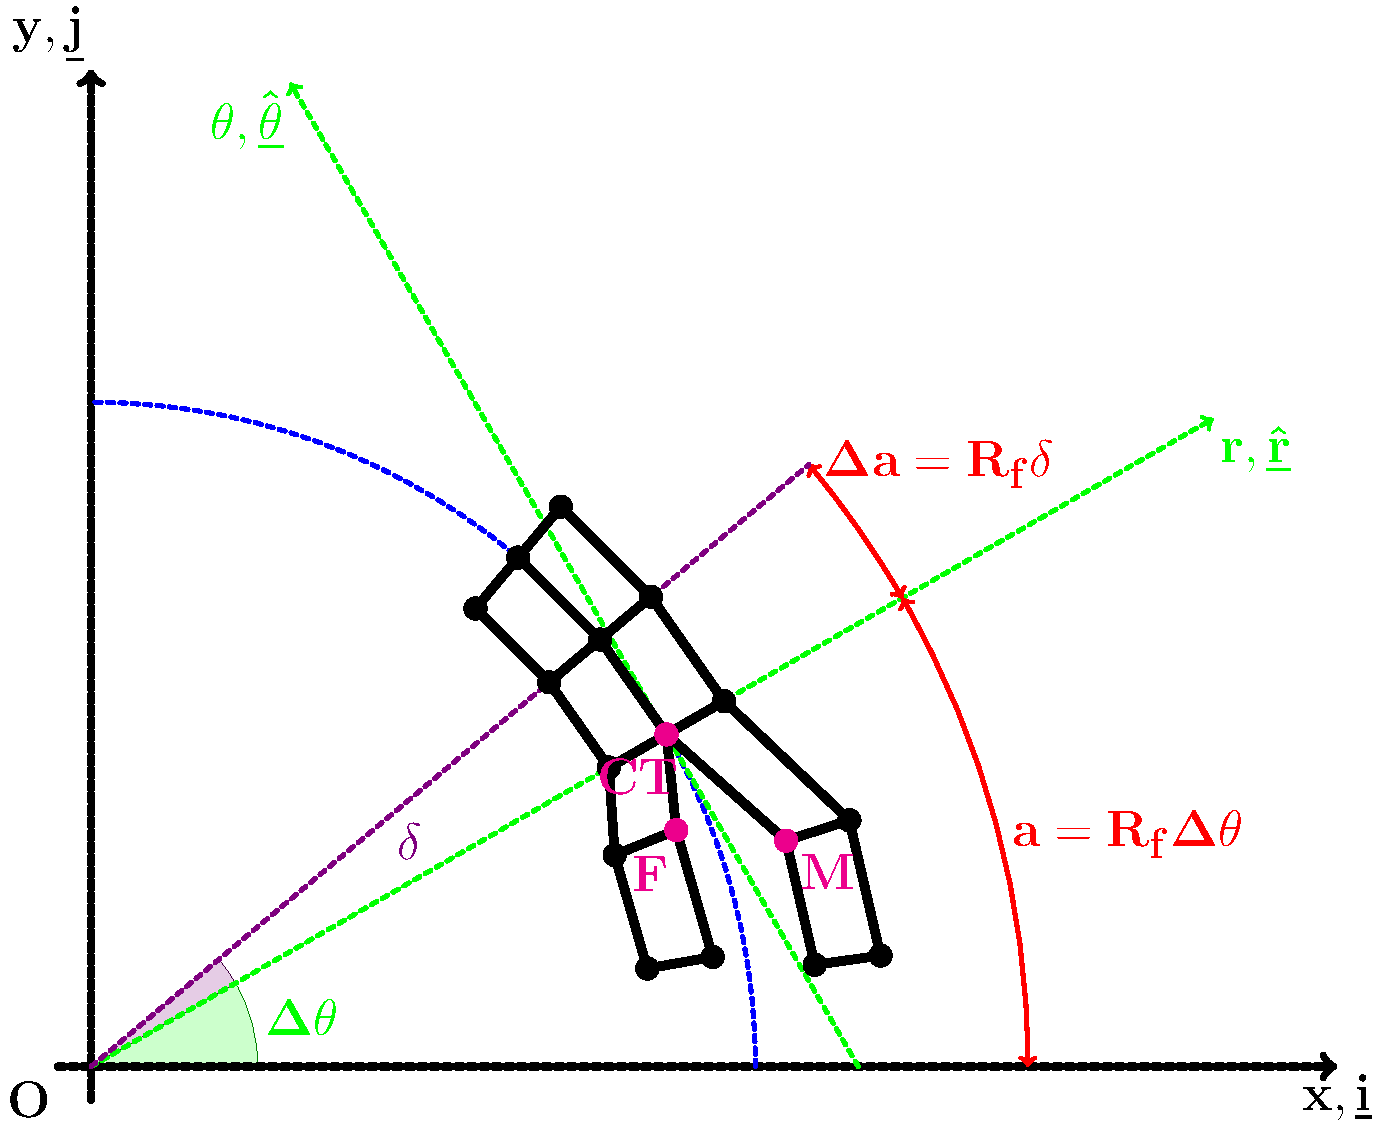
\includegraphics[width=\textwidth]{VCCT-linear.pdf}
\caption{Schematic representation of the discretized crack tip geometry for  $1^{st}$ order quadrilateral elements.}
\end{figure}

\begin{equation}
\underline{\underline{R}}=\begin{bmatrix}
\cos\left(\Delta\theta\right) & \sin\left(\Delta\theta\right) \\
-\sin\left(\Delta\theta\right) & \cos\left(\Delta\theta\right)
\end{bmatrix}\qquad\underline{\underline{R}}^{-1}=\underline{\underline{R}}^{T}=\begin{bmatrix}
\cos\left(\Delta\theta\right) & -\sin\left(\Delta\theta\right) \\
\sin\left(\Delta\theta\right) & \cos\left(\Delta\theta\right)
\end{bmatrix}
\end{equation}

\begin{equation}
\begin{bmatrix}
r \\
\theta
\end{bmatrix}=\underline{\underline{R}}\begin{bmatrix}
x \\
y
\end{bmatrix}\qquad\begin{bmatrix}
x \\
y
\end{bmatrix}=\underline{\underline{R}}^{-1}\begin{bmatrix}
r \\
\theta
\end{bmatrix}
\end{equation}

\subsection{Calculation of displacements and reaction forces}

\begin{equation}
u_{x}=u_{x,M}-u_{x,F}\qquad u_{y}=u_{y,M}-u_{y,F}
\end{equation}

\begin{equation}
u_{r}=\cos\left(\Delta\theta\right) u_{x}+\sin\left(\Delta\theta\right) u_{y}\qquad u_{\theta}=-\sin\left(\Delta\theta\right) u_{x}+\cos\left(\Delta\theta\right) u_{y}
\end{equation}

\begin{equation}
F_{r}=\cos\left(\Delta\theta\right) F_{x,CT}+\sin\left(\Delta\theta\right) F_{y,CT}\qquad F_{\theta}=-\sin\left(\Delta\theta\right) F_{x,CT}+\cos\left(\Delta\theta\right) F_{y,CT}
\end{equation}

\subsection{Calculation of energy release rates}

\begin{equation}
\begin{split}
G_{I,r\theta} = &\frac{1}{2}\frac{F_{r}u_{r}}{R_{f}\delta}=\\
= &\frac{1}{2R_{f}\delta}\left(\cos\left(\Delta\theta\right) F_{x}+\sin\left(\Delta\theta\right)F_{y}\right)\left(\cos\left(\Delta\theta\right) u_{x}+\sin\left(\Delta\theta\right) u_{y}\right)=\\
= &\frac{1}{2R_{f}\delta}\left(\cos^{2}\left(\Delta\theta\right) F_{x}u_{x}+\left(F_{x}u_{y}+F_{y}u_{x}\right)\cos\left(\Delta\theta\right)\sin\left(\Delta\theta\right)+\sin^{2}\left(\Delta\theta\right)F_{y}u_{y}\right)\\
\end{split}
\end{equation}

\begin{equation}
\begin{split}
G_{II,r\theta} = &\frac{1}{2}\frac{F_{\theta}u_{\theta}}{R_{f}\delta}=\\
= &\frac{1}{2R_{f}\delta}\left(-\sin\left(\Delta\theta\right) F_{x}+\cos\left(\Delta\theta\right)F_{y}\right)\left(-\sin\left(\Delta\theta\right) u_{x}+\cos\left(\Delta\theta\right) u_{y}\right)=\\
= &\frac{1}{2R_{f}\delta}\left(\sin^{2}\left(\Delta\theta\right) F_{x}u_{x}-\left(F_{x}u_{y}+F_{y}u_{x}\right)\cos\left(\Delta\theta\right)\sin\left(\Delta\theta\right)+\cos^{2}\left(\Delta\theta\right)F_{y}u_{y}\right)\\
\end{split}
\end{equation}

\begin{equation}
\begin{split}
G_{TOT,r\theta} = &G_{I,r\theta} + G_{II,r\theta}=\\
= &\frac{1}{2R_{f}\delta}\left(\cos^{2}\left(\Delta\theta\right) F_{x}u_{x}+\left(F_{x}u_{y}+F_{y}u_{x}\right)\cos\left(\Delta\theta\right)\sin\left(\Delta\theta\right)+\sin^{2}\left(\Delta\theta\right)F_{y}u_{y}\right)+\\
&+ \frac{1}{2R_{f}\delta}\left(\sin^{2}\left(\Delta\theta\right) F_{x}u_{x}-\left(F_{x}u_{y}+F_{y}u_{x}\right)\cos\left(\Delta\theta\right)\sin\left(\Delta\theta\right)+\cos^{2}\left(\Delta\theta\right)F_{y}u_{y}\right)=\\
=&\frac{1}{2R_{f}\delta}\left(\cancelto{1}{\left(\cos^{2}\left(\Delta\theta\right)+\sin^{2}\left(\Delta\theta\right)\right)}F_{x}u_{x}\right)+\\
&+\frac{1}{2R_{f}\delta}\left(\cancelto{0}{\left(\left(F_{x}u_{y}+F_{y}u_{x}\right)-\left(F_{x}u_{y}+F_{y}u_{x}\right)\right)}\cos\left(\Delta\theta\right)\sin\left(\Delta\theta\right)\right)+\\
&+\frac{1}{2R_{f}\delta}\left(\cancelto{1}{\left(\cos^{2}\left(\Delta\theta\right)+\sin^{2}\left(\Delta\theta\right)\right)}F_{y}u_{y}\right)=\\
=&\frac{1}{2}\frac{F_{x}u_{x}}{R_{f}\delta}+\frac{1}{2}\frac{F_{y}u_{y}}{R_{f}\delta}=\\
=&\widetilde{G}_{I,xy} + \widetilde{G}_{II,xy}=\widetilde{G}_{TOT,xy}
\end{split}
\end{equation}

\begin{equation}
\begin{split}
G_{I,r\theta} =&\frac{1}{2R_{f}\delta}\left(\cos^{2}\left(\Delta\theta\right) F_{x}u_{x}+\left(F_{x}u_{y}+F_{y}u_{x}\right)\cos\left(\Delta\theta\right)\sin\left(\Delta\theta\right)+\sin^{2}\left(\Delta\theta\right)F_{y}u_{y}\right)=\\
=&\cos^{2}\left(\Delta\theta\right)\frac{ F_{x}u_{x}}{2R_{f}\delta}+\left(\frac{F_{x}u_{y}}{2R_{f}\delta}+\frac{F_{y}u_{x}}{2R_{f}\delta}\right)\cos\left(\Delta\theta\right)\sin\left(\Delta\theta\right)+\sin^{2}\left(\Delta\theta\right)\frac{F_{y}u_{y}}{2R_{f}\delta}=\\
=&\cos^{2}\left(\Delta\theta\right)\widetilde{G}_{I,xy}+\left(\widetilde{G}_{I,xy}\frac{u_{y}}{u_{x}}+\widetilde{G}_{II,xy}\frac{u_{x}}{u_{y}}\right)\cos\left(\Delta\theta\right)\sin\left(\Delta\theta\right)+\sin^{2}\left(\Delta\theta\right)\widetilde{G}_{II,xy}
\end{split}
\end{equation}

\begin{equation}
\begin{split}
G_{II,r\theta} =&\frac{1}{2R_{f}\delta}\left(\sin^{2}\left(\Delta\theta\right) F_{x}u_{x}-\left(F_{x}u_{y}+F_{y}u_{x}\right)\cos\left(\Delta\theta\right)\sin\left(\Delta\theta\right)+\cos^{2}\left(\Delta\theta\right)F_{y}u_{y}\right)=\\
=&\sin^{2}\left(\Delta\theta\right)\frac{ F_{x}u_{x}}{2R_{f}\delta}-\left(\frac{F_{x}u_{y}}{2R_{f}\delta}+\frac{F_{y}u_{x}}{2R_{f}\delta}\right)\cos\left(\Delta\theta\right)\sin\left(\Delta\theta\right)+\cos^{2}\left(\Delta\theta\right)\frac{F_{y}u_{y}}{2R_{f}\delta}=\\
=&\sin^{2}\left(\Delta\theta\right)\widetilde{G}_{I,xy}-\left(\widetilde{G}_{I,xy}\frac{u_{y}}{u_{x}}+\widetilde{G}_{II,xy}\frac{u_{x}}{u_{y}}\right)\cos\left(\Delta\theta\right)\sin\left(\Delta\theta\right)+\cos^{2}\left(\Delta\theta\right)\widetilde{G}_{II,xy}
\end{split}
\end{equation}

\subsection{Sensitivity analysis of the FEM solution}

\begin{equation}
F_{x}\sim k_{x}u_{x}\qquad F_{y}\sim k_{y}u_{y}
\end{equation}

\begin{equation}
\begin{split}
G_{I,r\theta} \sim&\frac{1}{2R_{f}\delta}\cos^{2}\left(\Delta\theta\right) k_{x}u^{2}_{x}\left(\Delta\theta\right)+\\
&+\frac{1}{2R_{f}\delta}\left(k_{x}+k_{y}\right)u_{x}\left(\Delta\theta\right)u_{y}\left(\Delta\theta\right)\cos\left(\Delta\theta\right)\sin\left(\Delta\theta\right)+\\
&+\frac{1}{2R_{f}\delta}\sin^{2}\left(\Delta\theta\right)k_{y}u^{2}_{y}\left(\Delta\theta\right)
\end{split}
\end{equation}

\begin{equation}
\begin{split}
G_{II,r\theta} \sim&\frac{1}{2R_{f}\delta}\sin^{2}\left(\Delta\theta\right) k_{x}u^{2}_{x}\left(\Delta\theta\right)+\\
&-\frac{1}{2R_{f}\delta}\left(k_{x}+k_{y}\right)u_{x}\left(\Delta\theta\right)u_{y}\left(\Delta\theta\right)\cos\left(\Delta\theta\right)\sin\left(\Delta\theta\right)+\\
&+\frac{1}{2R_{f}\delta}\cos^{2}\left(\Delta\theta\right)k_{y}u^{2}_{y}\left(\Delta\theta\right)
\end{split}
\end{equation}

\begin{equation}
G_{TOT,r\theta} \sim\frac{1}{2R_{f}\delta}\left( k_{x}u^{2}_{x}\left(\Delta\theta\right)+ k_{y}u^{2}_{y}\left(\Delta\theta\right)\right)
\end{equation}

\begin{equation}
\begin{split}
\frac{\partial G_{I,r\theta}}{\partial\Delta\theta} \sim&\frac{1}{R_{f}\delta}\cos^{2}\left(\Delta\theta\right) k_{x}u_{x}\left(\Delta\theta\right)\frac{\partial u_{x}\left(\Delta\theta\right)}{\partial\Delta\theta}+\\
&+\frac{1}{2R_{f}\delta}\left(k_{x}+k_{y}\right)\left(\frac{\partial u_{x}\left(\Delta\theta\right)}{\partial\Delta\theta}u_{y}\left(\Delta\theta\right)+u_{x}\left(\Delta\theta\right)\frac{\partial u_{y}\left(\Delta\theta\right)}{\partial\Delta\theta}\right)\cos\left(\Delta\theta\right)\sin\left(\Delta\theta\right)+\\
&+\frac{1}{R_{f}\delta}\sin^{2}\left(\Delta\theta\right)k_{y}u_{y}\left(\Delta\theta\right)\frac{\partial u_{y}\left(\Delta\theta\right)}{\partial\Delta\theta}+\\
&+\frac{1}{2R_{f}\delta}\left(k_{y}u^{2}_{y}\left(\Delta\theta\right)- k_{x}u^{2}_{x}\left(\Delta\theta\right)\right)\sin\left(2\Delta\theta\right)+\\
&+\frac{1}{2R_{f}\delta}\left(k_{x}u_{x}\left(\Delta\theta\right)u_{y}\left(\Delta\theta\right)+k_{y}u_{y}\left(\Delta\theta\right)u_{x}\left(\Delta\theta\right)\right)\cos\left(2\Delta\theta\right)\\
\end{split}
\end{equation}

\begin{equation}
\begin{split}
\frac{\partial G_{II,r\theta}}{\partial\Delta\theta} \sim&\frac{1}{R_{f}\delta}\sin^{2}\left(\Delta\theta\right) k_{x}u_{x}\left(\Delta\theta\right)\frac{\partial u_{x}\left(\Delta\theta\right)}{\partial\Delta\theta}+\\
&-\frac{1}{2R_{f}\delta}\left(k_{x}+k_{y}\right)\left(\frac{\partial u_{x}\left(\Delta\theta\right)}{\partial\Delta\theta}u_{y}\left(\Delta\theta\right)+u_{x}\left(\Delta\theta\right)\frac{\partial u_{y}\left(\Delta\theta\right)}{\partial\Delta\theta}\right)\cos\left(\Delta\theta\right)\sin\left(\Delta\theta\right)+\\
&+\frac{1}{R_{f}\delta}\cos^{2}\left(\Delta\theta\right)k_{y}u_{y}\left(\Delta\theta\right)\frac{\partial u_{y}\left(\Delta\theta\right)}{\partial\Delta\theta}+\\
&+\frac{1}{2R_{f}\delta}\left(k_{x}u^{2}_{x}\left(\Delta\theta\right)- k_{y}u^{2}_{y}\left(\Delta\theta\right)\right)\sin\left(2\Delta\theta\right)+\\
&-\frac{1}{2R_{f}\delta}\left(k_{x}u_{x}\left(\Delta\theta\right)u_{y}\left(\Delta\theta\right)+k_{y}u_{y}\left(\Delta\theta\right)u_{x}\left(\Delta\theta\right)\right)\cos\left(2\Delta\theta\right)\\
\end{split}
\end{equation}

\begin{equation}
\frac{\partial G_{TOT,r\theta}}{\partial\Delta\theta} \sim\frac{1}{R_{f}\delta}\left( k_{x}u_{x}\left(\Delta\theta\right)\frac{\partial u_{x}\left(\Delta\theta\right)}{\partial\Delta\theta}+ k_{y}u_{y}\left(\Delta\theta\right)\frac{\partial u_{y}\left(\Delta\theta\right)}{\partial\Delta\theta}\right)
\end{equation}

\clearpage

%------------------------------------------------------------------------------------------%
%                             VCCT 2nd order
%------------------------------------------------------------------------------------------%

\section{VCCT for second order quadrilateral elements}

\subsection{Definition of crack tip reference frame}

\begin{figure}[!h]
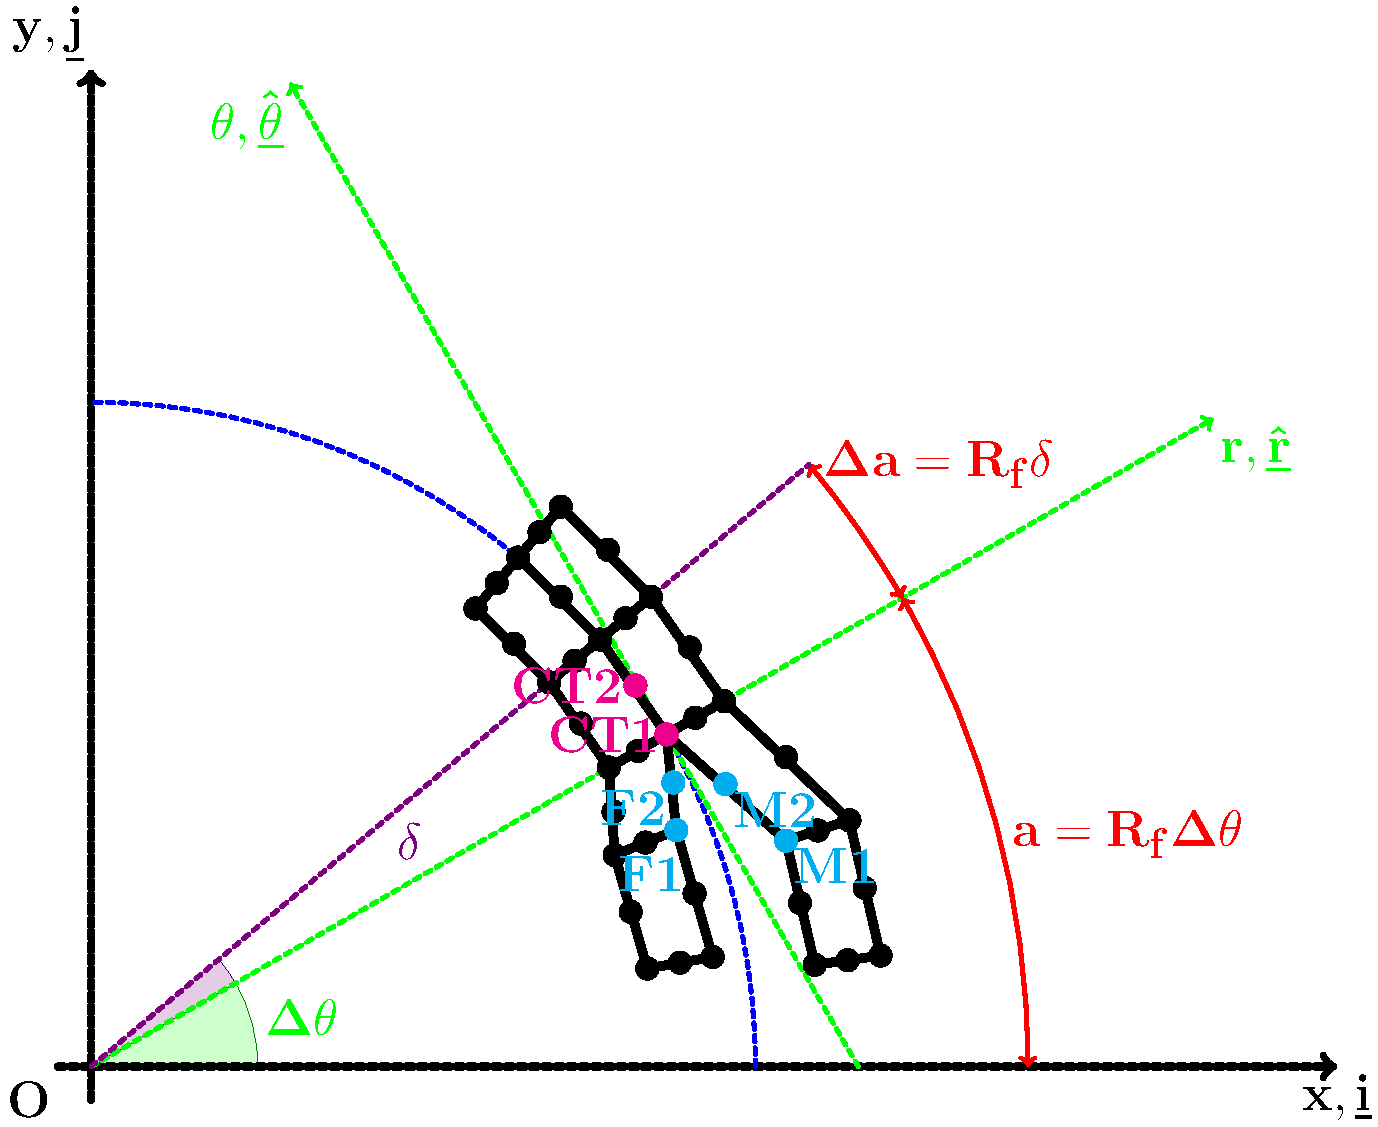
\includegraphics[width=\textwidth]{VCCT-quadratic.pdf}
\caption{Schematic representation of the discretized crack tip geometry for $2^{nd}$ order quadrilateral elements.}
\end{figure}

\begin{equation}
\underline{\underline{R}}=\begin{bmatrix}
\cos\left(\Delta\theta\right) & \sin\left(\Delta\theta\right) \\
-\sin\left(\Delta\theta\right) & \cos\left(\Delta\theta\right)
\end{bmatrix}\qquad\underline{\underline{R}}^{-1}=\underline{\underline{R}}^{T}=\begin{bmatrix}
\cos\left(\Delta\theta\right) & -\sin\left(\Delta\theta\right) \\
\sin\left(\Delta\theta\right) & \cos\left(\Delta\theta\right)
\end{bmatrix}
\end{equation}

\begin{equation}
\begin{bmatrix}
r \\
\theta
\end{bmatrix}=\underline{\underline{R}}\begin{bmatrix}
x \\
y
\end{bmatrix}\qquad\begin{bmatrix}
x \\
y
\end{bmatrix}=\underline{\underline{R}}^{-1}\begin{bmatrix}
r \\
\theta
\end{bmatrix}
\end{equation}

\subsection{Calculation of displacements and reaction forces}

\begin{equation}
\begin{split}
u_{x,1}=u_{x,M1}-u_{x,F1}&\qquad u_{y,1}=u_{y,M1}-u_{y,F1}\\
u_{x,2}=u_{x,M2}-u_{x,F2}&\qquad u_{y,2}=u_{y,M2}-u_{y,F2}
\end{split}
\end{equation}

\begin{equation}
\begin{split}
u_{r,1}=\cos\left(\Delta\theta\right) u_{x,1}+\sin\left(\Delta\theta\right) u_{y,1}&\qquad u_{\theta,1}=-\sin\left(\Delta\theta\right) u_{x,1}+\cos\left(\Delta\theta\right) u_{y,1}\\
u_{r,2}=\cos\left(\Delta\theta\right) u_{x,2}+\sin\left(\Delta\theta\right) u_{y,2}&\qquad u_{\theta,2}=-\sin\left(\Delta\theta\right) u_{x,2}+\cos\left(\Delta\theta\right) u_{y,2}
\end{split}
\end{equation}

\begin{equation}
\begin{split}
F_{r,1}=\cos\left(\Delta\theta\right) F_{x,1}+\sin\left(\Delta\theta\right) F_{y,1}&\qquad F_{\theta,1}=-\sin\left(\Delta\theta\right) F_{x,1}+\cos\left(\Delta\theta\right) F_{y,1}\\
F_{r,2}=\cos\left(\Delta\theta\right) F_{x,2}+\sin\left(\Delta\theta\right) F_{y,2}&\qquad F_{\theta,2}=-\sin\left(\Delta\theta\right) F_{x,2}+\cos\left(\Delta\theta\right) F_{y,2}\\
\end{split}
\end{equation}

\subsection{Calculation of energy release rates}

\begin{equation}
\begin{split}
G_{I,r\theta} = &\frac{1}{2R_{f}\delta}\left(F_{r,1}u_{r,1}+F_{r,2}u_{r,2}\right)=\\
= &\frac{1}{2R_{f}\delta}\left(\cos\left(\Delta\theta\right) F_{x,1}+\sin\left(\Delta\theta\right)F_{y,1}\right)\left(\cos\left(\Delta\theta\right) u_{x,1}+\sin\left(\Delta\theta\right) u_{y,1}\right)+\\
&+\frac{1}{2R_{f}\delta}\left(\cos\left(\Delta\theta\right) F_{x,2}+\sin\left(\Delta\theta\right)F_{y,2}\right)\left(\cos\left(\Delta\theta\right) u_{x,2}+\sin\left(\Delta\theta\right) u_{y,2}\right)+\\
= &\frac{1}{2R_{f}\delta}\left(\cos^{2}\left(\Delta\theta\right) F_{x,1}u_{x,1}+\left(F_{x,1}u_{y,1}+F_{y,1}u_{x,1}\right)\cos\left(\Delta\theta\right)\sin\left(\Delta\theta\right)+\sin^{2}\left(\Delta\theta\right)F_{y,1}u_{y,1}\right)+\\
&+\frac{1}{2R_{f}\delta}\left(\cos^{2}\left(\Delta\theta\right) F_{x,2}u_{x,2}+\left(F_{x,2}u_{y,2}+F_{y,2}u_{x,2}\right)\cos\left(\Delta\theta\right)\sin\left(\Delta\theta\right)+\sin^{2}\left(\Delta\theta\right)F_{y,2}u_{y,2}\right)
\end{split}
\end{equation}

\begin{equation}
\begin{split}
G_{II,r\theta} = &\frac{1}{2R_{f}\delta}\left(F_{\theta,1}u_{\theta,1}+F_{\theta,2}u_{\theta,2}\right)=\\
= &\frac{1}{2R_{f}\delta}\left(-\sin\left(\Delta\theta\right) F_{x,1}+\cos\left(\Delta\theta\right)F_{y,1}\right)\left(-\sin\left(\Delta\theta\right) u_{x,1}+\cos\left(\Delta\theta\right) u_{y,1}\right)+\\
&+\frac{1}{2R_{f}\delta}\left(-\sin\left(\Delta\theta\right) F_{x,2}+\cos\left(\Delta\theta\right)F_{y,2}\right)\left(-\sin\left(\Delta\theta\right) u_{x,2}+\cos\left(\Delta\theta\right) u_{y,2}\right)=\\
= &\frac{1}{2R_{f}\delta}\left(\sin^{2}\left(\Delta\theta\right) F_{x,1}u_{x,1}-\left(F_{x,1}u_{y,1}+F_{y,1}u_{x,1}\right)\cos\left(\Delta\theta\right)\sin\left(\Delta\theta\right)+\cos^{2}\left(\Delta\theta\right)F_{y,1}u_{y,1}\right)+\\
 &+\frac{1}{2R_{f}\delta}\left(\sin^{2}\left(\Delta\theta\right) F_{x,2}u_{x,2}-\left(F_{x,2}u_{y,2}+F_{y,2}u_{x,2}\right)\cos\left(\Delta\theta\right)\sin\left(\Delta\theta\right)+\cos^{2}\left(\Delta\theta\right)F_{y,2}u_{y,2}\right)\\
\end{split}
\end{equation}

\begin{equation}
\begin{split}
G_{TOT,r\theta} = &G_{I,r\theta} + G_{II,r\theta}=\\
=&\frac{1}{2R_{f}\delta}\left(\cos^{2}\left(\Delta\theta\right) F_{x,1}u_{x,1}+\left(F_{x,1}u_{y,1}+F_{y,1}u_{x,1}\right)\cos\left(\Delta\theta\right)\sin\left(\Delta\theta\right)+\sin^{2}\left(\Delta\theta\right)F_{y,1}u_{y,1}\right)+\\
&+\frac{1}{2R_{f}\delta}\left(\cos^{2}\left(\Delta\theta\right) F_{x,2}u_{x,2}+\left(F_{x,2}u_{y,2}+F_{y,2}u_{x,2}\right)\cos\left(\Delta\theta\right)\sin\left(\Delta\theta\right)+\sin^{2}\left(\Delta\theta\right)F_{y,2}u_{y,2}\right)+\\
&+\frac{1}{2R_{f}\delta}\left(\sin^{2}\left(\Delta\theta\right) F_{x,1}u_{x,1}-\left(F_{x,1}u_{y,1}+F_{y,1}u_{x,1}\right)\cos\left(\Delta\theta\right)\sin\left(\Delta\theta\right)+\cos^{2}\left(\Delta\theta\right)F_{y,1}u_{y,1}\right)+\\
 &+\frac{1}{2R_{f}\delta}\left(\sin^{2}\left(\Delta\theta\right) F_{x,2}u_{x,2}-\left(F_{x,2}u_{y,2}+F_{y,2}u_{x,2}\right)\cos\left(\Delta\theta\right)\sin\left(\Delta\theta\right)+\cos^{2}\left(\Delta\theta\right)F_{y,2}u_{y,2}\right)=\\
= &\frac{1}{2R_{f}\delta}\cos^{2}\left(\Delta\theta\right) \left(F_{x,1}u_{x,1}+F_{x,2}u_{x,2}+F_{y,1}u_{y,1}+F_{y,2}u_{y,2}\right)+\\
&+\frac{1}{2R_{f}\delta}\left(\left(F_{x,1}u_{y,1}+F_{x,1}u_{y,1}\right)+\left(F_{y,2}u_{x,2}+F_{y,2}u_{x,2}\right)\right)\cos\left(\Delta\theta\right)\sin\left(\Delta\theta\right)+\\
&+\frac{1}{2R_{f}\delta}\sin^{2}\left(\Delta\theta\right)\left(F_{x,1}u_{x,1}+F_{x,2}u_{x,2}+F_{y,1}u_{y,1}+F_{y,2}u_{y,2}\right)+\\
&-\frac{1}{2R_{f}\delta}\left(\left(F_{x,1}u_{y,1}+F_{x,1}u_{y,1}\right)+\left(F_{y,2}u_{x,2}+F_{y,2}u_{x,2}\right)\right)\cos\left(\Delta\theta\right)\sin\left(\Delta\theta\right)=\\
=&\frac{1}{2R_{f}\delta}\left(\cancelto{1}{\left(\cos^{2}\left(\Delta\theta\right)+\sin^{2}\left(\Delta\theta\right)\right)}\left(F_{x,1}u_{x,1}+F_{x,2}u_{x,2}\right)\right)+\\
&+\frac{1}{2R_{f}\delta}\cancelto{0}{\left(\left(F_{x,1}u_{y,1}+F_{x,1}u_{y,1}\right)-\left(F_{x,1}u_{y,1}+F_{x,1}u_{y,1}\right)\right)}\cos\left(\Delta\theta\right)\sin\left(\Delta\theta\right)+\\
&+\frac{1}{2R_{f}\delta}\cancelto{0}{\left(\left(F_{y,2}u_{x,2}+F_{y,2}u_{x,2}\right)-\left(F_{y,2}u_{x,2}+F_{y,2}u_{x,2}\right)\right)}\cos\left(\Delta\theta\right)\sin\left(\Delta\theta\right)+\\
&+\frac{1}{2R_{f}\delta}\left(\cancelto{1}{\left(\cos^{2}\left(\Delta\theta\right)+\sin^{2}\left(\Delta\theta\right)\right)}\left(F_{y,1}u_{y,1}+F_{y,2}u_{y,2}\right)\right)=\\
=&\frac{1}{2}\frac{F_{x,1}u_{x,1}+F_{x,2}u_{x,2}}{R_{f}\delta}+\frac{1}{2}\frac{F_{y,1}u_{y,1}+F_{y,2}u_{y,2}}{R_{f}\delta}=\\
=&\widetilde{G}_{I,xy} + \widetilde{G}_{II,xy}=\widetilde{G}_{TOT,xy}
\end{split}
\end{equation}

\begin{equation}
\begin{split}
G_{I,r\theta} = &\cos^{2}\left(\Delta\theta\right)\frac{F_{x,1}u_{x,1}+F_{x,2}u_{x,2}}{2R_{f}\delta}+\\
&+\frac{F_{x,1}u_{y,1}+F_{y,1}u_{x,1}+F_{x,2}u_{y,2}+F_{y,2}u_{x,2}}{2R_{f}\delta}\cos\left(\Delta\theta\right)\sin\left(\Delta\theta\right)+\\
&+\sin^{2}\left(\Delta\theta\right)\frac{F_{y,1}u_{y,1}+F_{y,2}u_{y,2}}{2R_{f}\delta}=\\
=&\cos^{2}\left(\Delta\theta\right)\widetilde{G}_{I,xy}+\sin^{2}\left(\Delta\theta\right)\widetilde{G}_{II,xy}+\\
&+\frac{F_{x,1}u_{y,1}+F_{y,1}u_{x,1}+F_{x,2}u_{y,2}+F_{y,2}u_{x,2}}{2R_{f}\delta}\cos\left(\Delta\theta\right)\sin\left(\Delta\theta\right)
\end{split}
\end{equation}

\begin{equation}
\begin{split}
G_{II,r\theta} = &\sin^{2}\left(\Delta\theta\right)\frac{F_{x,1}u_{x,1}+F_{x,2}u_{x,2}}{2R_{f}\delta}+\\
&-\frac{F_{x,1}u_{y,1}+F_{y,1}u_{x,1}+F_{x,2}u_{y,2}+F_{y,2}u_{x,2}}{2R_{f}\delta}\cos\left(\Delta\theta\right)\sin\left(\Delta\theta\right)+\\
&+\cos^{2}\left(\Delta\theta\right)\frac{F_{y,1}u_{y,1}+F_{y,2}u_{y,2}}{2R_{f}\delta}=\\
=&\sin^{2}\left(\Delta\theta\right)\widetilde{G}_{I,xy}+\cos^{2}\left(\Delta\theta\right)\widetilde{G}_{II,xy}+\\
&-\frac{F_{x,1}u_{y,1}+F_{y,1}u_{x,1}+F_{x,2}u_{y,2}+F_{y,2}u_{x,2}}{2R_{f}\delta}\cos\left(\Delta\theta\right)\sin\left(\Delta\theta\right)
\end{split}
\end{equation}

\subsection{Sensitivity analysis of the FEM solution}

\begin{equation}
\begin{split}
F_{x,1}\sim k_{x,1}u_{x,1}&\qquad F_{y,1}\sim k_{y,1}u_{y,1}\\
F_{x,2}\sim k_{x,2}u_{x,2}&\qquad F_{y,2}\sim k_{y,2}u_{y,2}\\
\end{split}
\end{equation}

\begin{equation}
\begin{split}
G_{I,r\theta} \sim &\frac{1}{2R_{f}\delta}\cos^{2}\left(\Delta\theta\right)\left(k_{x,1}u^{2}_{x,1}+k_{x,2}u^{2}_{x,2}\right)+\\
&+\frac{1}{2R_{f}\delta}\cos\left(\Delta\theta\right)\sin\left(\Delta\theta\right)\left(k_{x,1}u_{x,1}u_{y,1}+k_{y,1}u_{y,1}u_{x,1}+k_{x,2}u_{x,2}u_{y,2}+k_{y,2}u_{y,2}u_{x,2}\right)+\\
&+\frac{1}{2R_{f}\delta}\sin^{2}\left(\Delta\theta\right)\left(k_{y,1}u^{2}_{y,1}+k_{y,2}u^{2}_{y,2}\right)
\end{split}
\end{equation}

\begin{equation}
\begin{split}
G_{II,r\theta} \sim &\frac{1}{2R_{f}\delta}\sin^{2}\left(\Delta\theta\right)\left(k_{x,1}u^{2}_{x,1}+k_{x,2}u^{2}_{x,2}\right)+\\
&-\frac{1}{2R_{f}\delta}\cos\left(\Delta\theta\right)\sin\left(\Delta\theta\right)\left(k_{x,1}u_{x,1}u_{y,1}+k_{y,1}u_{y,1}u_{x,1}+k_{x,2}u_{x,2}u_{y,2}+k_{y,2}u_{y,2}u_{x,2}\right)+\\
&+\frac{1}{2R_{f}\delta}\cos^{2}\left(\Delta\theta\right)\left(k_{y,1}u^{2}_{y,1}+k_{y,2}u^{2}_{y,2}\right)
\end{split}
\end{equation}

\begin{equation}
\begin{split}
G_{TOT,r\theta} \sim &\frac{1}{2R_{f}\delta}\left(\left(k_{x,1}u^{2}_{x,1}\left(\Delta\theta\right)+k_{x,2}u^{2}_{x,2}\left(\Delta\theta\right)\right)+\left(k_{y,1}u^{2}_{y,1}\left(\Delta\theta\right)+k_{y,2}u^{2}_{y,2}\left(\Delta\theta\right)\right)\right)
\end{split}
\end{equation}

\begin{equation}
\begin{split}
\frac{\partial G_{I,r\theta}}{\partial\Delta\theta} \sim&\frac{1}{R_{f}\delta}\cos^{2}\left(\Delta\theta\right)\left( k_{x,1}u_{x,1}\left(\Delta\theta\right)\frac{\partial u_{x,1}\left(\Delta\theta\right)}{\partial\Delta\theta}+k_{x,2}u_{x,2}\left(\Delta\theta\right)\frac{\partial u_{x,2}\left(\Delta\theta\right)}{\partial\Delta\theta}\right)+\\
&+\frac{1}{2R_{f}\delta}\left(k_{x,1}+k_{y,1}\right)\left(\frac{\partial u_{x,1}\left(\Delta\theta\right)}{\partial\Delta\theta}u_{y,1}\left(\Delta\theta\right)+u_{x,1}\left(\Delta\theta\right)\frac{\partial u_{y,1}\left(\Delta\theta\right)}{\partial\Delta\theta}\right)\cos\left(\Delta\theta\right)\sin\left(\Delta\theta\right)+\\
&+\frac{1}{2R_{f}\delta}\left(k_{x,2}+k_{y,2}\right)\left(\frac{\partial u_{x,2}\left(\Delta\theta\right)}{\partial\Delta\theta}u_{y,2}\left(\Delta\theta\right)+u_{x,2}\left(\Delta\theta\right)\frac{\partial u_{y,2}\left(\Delta\theta\right)}{\partial\Delta\theta}\right)\cos\left(\Delta\theta\right)\sin\left(\Delta\theta\right)+\\
&+\frac{1}{R_{f}\delta}\sin^{2}\left(\Delta\theta\right)\left(k_{y,1}u_{y,1}\left(\Delta\theta\right)\frac{\partial u_{y,1}\left(\Delta\theta\right)}{\partial\Delta\theta}+k_{y,2}u_{y,2}\left(\Delta\theta\right)\frac{\partial u_{y,2}\left(\Delta\theta\right)}{\partial\Delta\theta}\right)+\\
&+\frac{1}{2R_{f}\delta}\left(\left(k_{y,1}u^{2}_{y,1}+k_{y,2}u^{2}_{y,2}\right)-\left(k_{x,1}u^{2}_{x,1}+k_{x,2}u^{2}_{x,2}\right)\right)\sin\left(2\Delta\theta\right)+\\
&+\frac{1}{2R_{f}\delta}\left(\left(k_{x,1}+k_{y,1}\right)u_{x,1}u_{y,1}+\left(k_{x,2}+k_{y,2}\right)u_{x,2}u_{y,2}\right)\cos\left(2\Delta\theta\right)\\
\end{split}
\end{equation}

\begin{equation}
\begin{split}
\frac{\partial G_{II,r\theta}}{\partial\Delta\theta} \sim&\frac{1}{R_{f}\delta}\sin^{2}\left(\Delta\theta\right)\left( k_{x,1}u_{x,1}\left(\Delta\theta\right)\frac{\partial u_{x,1}\left(\Delta\theta\right)}{\partial\Delta\theta}+k_{x,2}u_{x,2}\left(\Delta\theta\right)\frac{\partial u_{x,2}\left(\Delta\theta\right)}{\partial\Delta\theta}\right)+\\
&-\frac{1}{2R_{f}\delta}\left(k_{x,1}+k_{y,1}\right)\left(\frac{\partial u_{x,1}\left(\Delta\theta\right)}{\partial\Delta\theta}u_{y,1}\left(\Delta\theta\right)+u_{x,1}\left(\Delta\theta\right)\frac{\partial u_{y,1}\left(\Delta\theta\right)}{\partial\Delta\theta}\right)\cos\left(\Delta\theta\right)\sin\left(\Delta\theta\right)+\\
&-\frac{1}{2R_{f}\delta}\left(k_{x,2}+k_{y,2}\right)\left(\frac{\partial u_{x,2}\left(\Delta\theta\right)}{\partial\Delta\theta}u_{y,2}\left(\Delta\theta\right)+u_{x,2}\left(\Delta\theta\right)\frac{\partial u_{y,2}\left(\Delta\theta\right)}{\partial\Delta\theta}\right)\cos\left(\Delta\theta\right)\sin\left(\Delta\theta\right)+\\
&+\frac{1}{R_{f}\delta}\cos^{2}\left(\Delta\theta\right)\left(k_{y,1}u_{y,1}\left(\Delta\theta\right)\frac{\partial u_{y,1}\left(\Delta\theta\right)}{\partial\Delta\theta}+k_{y,2}u_{y,2}\left(\Delta\theta\right)\frac{\partial u_{y,2}\left(\Delta\theta\right)}{\partial\Delta\theta}\right)+\\
&+\frac{1}{2R_{f}\delta}\left(\left(k_{x,1}u^{2}_{x,1}+k_{x,2}u^{2}_{x,2}\right)-\left(k_{y,1}u^{2}_{y,1}+k_{y,2}u^{2}_{y,2}\right)\right)\sin\left(2\Delta\theta\right)+\\
&-\frac{1}{2R_{f}\delta}\left(\left(k_{x,1}+k_{y,1}\right)u_{x,1}u_{y,1}+\left(k_{x,2}+k_{y,2}\right)u_{x,2}u_{y,2}\right)\cos\left(2\Delta\theta\right)\\
\end{split}
\end{equation}

\begin{equation}
\begin{split}
G_{TOT,r\theta} \sim &\frac{1}{R_{f}\delta}\left(\left( k_{x,1}u_{x,1}\frac{\partial u_{x,1}}{\partial\Delta\theta}+k_{x,2}u_{x,2}\frac{\partial u_{x,2}}{\partial\Delta\theta}\right)+\left(k_{y,1}u_{y,1}\frac{\partial u_{y,1}}{\partial\Delta\theta}+k_{y,2}u_{y,2}\frac{\partial u_{y,2}}{\partial\Delta\theta}\right)\right)
\end{split}
\end{equation}

\clearpage

%------------------------------------------------------------------------------------------%
%                             Interpolation
%------------------------------------------------------------------------------------------%

\section{Trigonometric interpolation}

By inspecting the results of the previous sections, an interpolation of the BEM results is performed manually by trial and error. The following procedure is followed:

\begin{enumerate}
\item a basis function is selected;
\item the frequency of the trigonometric basis function is calculated based on the position of the maximum value; 
\item the amplitude is calculated based on the maximum value.
\end{enumerate}

\begin{figure}[!h]
\includegraphics[width=\textwidth]{Gsplot.pdf}
\caption{Interpolation of BEM results by manual trial and error.}
\end{figure}

The good agreement suggests that trigonometric functions are very good candidates for energy release rate data interpolation. The effect of different parameters can thus modeled as the functional variation of frequency (period) and amplitude of the trigonometric basis functions.

%\clearpage
%------------------------------------------------------------------------------------------%
%                             CONCLUSIONS AND PERSPECTIVES
%------------------------------------------------------------------------------------------%

%\section{Conclusions}


%------------------------------------------------------------------------------------------%
%                                   ACKNOWLEDGEMENTS
%------------------------------------------------------------------------------------------%
%\ack
%Luca Di Stasio gratefully acknowledges the support of the European School of Materials (EUSMAT) through the DocMASE Doctoral Programme and the European Commission through the Erasmus Mundus Programme.
%\newpage
%------------------------------------------------------------------------------------------%
%                                      REFERENCES
%------------------------------------------------------------------------------------------%
%\section*{References}
\begin{thebibliography}{9}
%\bibitem{author:year}author surname author initials (up to 10) year title {\it Journal} {\bf vol} (issue) pages
% Spread Tow Technology
\bibitem{spreadtowpatent:1974}Daniels C. Pneumatic spreading of filaments. USA: Space Systems/Loral LLC; 1974. USP 3795944.
\bibitem{spreadtowpatent:1991}Iyer S., Drzal L. T. Method and system for spreading a tow of fibers. USA: Michigan State University; 1991. USP 5042122.
\bibitem{spreadtowpatent:1992}Nakagawa, N., Ohsora, Y. Fiber separator for producing fiber reinforced metallic or resin body. Japan: Ube Industries Ltd; 1992. USP 5101542.
\bibitem{spreadtowpatent:2000}Lifke J. L., Busselle L. D., Finley D. J., Gordon B. W. Method and apparatus for spreading fiber bundles. USA: Adherent Tech Inc; 2000. USP 6049956.
\bibitem{spreadtowpatent:1993}Peritt J. M., Everett R., Edelstein A. Electrostatic fiber spreader including a corona discharge device. USA: US Secretary of Navy; 1993. USP 5200620.
\bibitem{KawabeTomodaMatsuo:1997}Kawabe K., Tomoda S. and Matsuo T. 1997 A pneumatic process for spreading reinforcing fiber tow {\it Proc. 42nd Int. SAMPE USA (Anaheim, CA, USA)} 65–76.
\bibitem{spreadtowpatent:2003}Kawabe K., Tomoda S. Method of producing a spread multi-filament bundle and an apparatus used in the same. Japan: Fukui Prefectural Government; 2003. JP 2003-193895.
\bibitem{Kawabe:2008} Kawabe K. 2008 New Spreading Technology for Carbon Fiber Tow and Its Application to Composite Materials {\it Sen'i Gakkaishi} {\bf 64} (8) 262--267 [in Japanese]
\bibitem{SasayamaTomoda:2009} Sasayama H. and Tomoda S. 2009 New Carbon Fiber Tow-Spread Technology and Applications to Advanced Composite Materials {\it S.A.M.P.E. journal} {\bf 45} (2) 6--17
\bibitem{ntpt}Meijer A. NTPT makes world’s thinnest prepeg even thinner [Internet] North Thin Ply Technology (NTPT) press release 2015 [cited 30 April 2017] Available from http://www.thinplytechnology.com/mesimages/Press\_Release\_NTPT-16JUN2015.pdf
\bibitem{oxeon}oXeon TECHNOLOGIES 2014 [Internet] [cited 30 April 2017] Available from http://oxeon.se/technologies/
% Experimental studies of thin plies and/or modeling
\bibitem{SihnKimKawabeTsai:2007}Sihn S., Kim R. Y., Kawabe K. and Tsai S. W. 2007 Experimental studies of thin-ply laminated composites {\it Compos. Sci. Technol.} {\bf 67} (6) 996--1008
\bibitem{SaitoTakeuchKimpara:2012}Saito H., Takeuchi H. and Kimpara I. 2012 Experimental Evaluation of the Damage Growth Restraining in $90^{\circ}$ Layer of Thin-ply CFRP Cross-ply Laminates {\it Adv. Compos. Mater.} {\bf 21} 57--66
\bibitem{ArteiroCatalanottiXavierCamanho:2013} Arteiro A., Catalanotti G., Xavier J. and Camanho P. P. 2013 Notched response of non-crimp fabric thin-ply laminates {\it Compos. Sci. Technol.} {\bf 79} 97--114
\bibitem{AmacherCugnoniBotsisSorensenSmithDransfeld:2014}Amacher R., Cugnoni J., Botsis J., Sorensen L., Smith W. and Dransfeld C. 2014 Thin ply composites: Experimental characterization and modeling of size-effects {\it Compos. Sci. Technol.} {\bf 101} 121--132
% Thin ply effect
\bibitem{ParviziBailey:1978}Parvizi A. and Bailey J. E. 1978 On multiple transverse cracking in glass fibre epoxy cross-ply laminates {\it J Mater Sci} {\bf 13} (10) 2121--2136
\bibitem{BaileyCurtisParvizi:1979}Bailey J. E., Curtis P. T. and Parvizi A. 1979 On the Transverse Cracking and Longitudinal Splitting Behaviour of Glass and Carbon Fibre Reinforced Epoxy Cross Ply Laminates and the Effect of Poisson and Thermally Generated Strain {\it Proc. R. Soc. London, Ser. A} {\bf 366} (1727) 599--623
\bibitem{FlaggsKural:1982}Flaggs D. L. and Kural M. H. 1982 Experimental Determination of the In Situ Transverse Lamina Strength in Graphite/Epoxy Laminates {\it J. Compos. Mater.} {\bf 16} (2) 103--116
% Modeling of thin plies
\bibitem{CamanhoDavilaPinhoIannucciRobinson:2006}Camanho P. P., D\'avila C. G., Pinho S. T., Iannucci L. and Robinson P. 2006 Prediction of in situ strengths and matrix cracking in composites under transverse tension and in-plane shear {\it Composites Part A} {\bf 37} (2) 165–176
\bibitem{SaitoTakehuchiKimpara:2014}Saito H., Takehuchi H. and Kimpara I. 2014 A study of crack suppression mechanism of thin-ply carbon-fiber-reinforced polymer laminate with mesoscopic numerical simulation {\it J. Compos. Mater.} {\bf 48} (17) 2085 - 2096
\bibitem{HerraezMoraNayaLopesGonzalezLLorca:2015}Herr\'aez M., Mora D., Naya F., Lopes C. S., Gonz\'alez C. and LLorca J. 2015 Transverse cracking of cross-ply laminates: A computational micromechanics perspective {\it Compos. Sci. Technol.} {\bf 110} 196--204
\bibitem{CanalGonzalezSeguradoLLorca:2012}Canal L. P., Gonz\'alez C., Segurado J. and LLorca J. 2012 Intraply fracture of fiber-reinforced composites: Microscopic mechanisms and modeling {\it Compos. Sci. Technol.} {\bf 72} (11) 1223--1232
% Representative Volume Element
\bibitem{Hill:1963}Hill R. 1963 Elastic properties of reinforced solids: Some theoretical principles {\it J. Mech. Ph. Solids} {\bf 11} (5) 357--372
\bibitem{SunVaidya:1996}Sun C. T. and Vaidya R. S. 1996 Prediction of composite properties from a representative volume element {\it Compos. Sci. Technol.} {\bf 56} (2) 171--179
\bibitem{Hashin:1983}Hashin Z. 1983 Analysis of Composite Materials -- A Survey {\it J. Appl. Mech} {\bf 50} (3) 481--505
\bibitem{Hashin:1962}Hashin Z. 1962 On some variational principles in anisotropic and nonhomogeneous elasticity {\it J. Mech. Ph. Solids} {\bf 10} (4) 335--342
\bibitem{Hashin:1963}Hashin Z. 1963 A variational approach to the theory of the elastic behaviour of multiphase materials {\it J. Mech. Ph. Solids} {\bf 11} (2) 127--140
\bibitem{SwaminathanGhoshPagano:2006}Swaminathan S., Ghosh S. and Pagano N. J. 2006 Statistically Equivalent Representative Volume Elements for Unidirectional Composite Microstructures: Part I - Without Damage {\it J. Compos. Mater.} {\bf 40} (7) 583--604
\bibitem{SwaminathanGhosh:2006}Swaminathan S.and Ghosh S. 2006 Statistically Equivalent Representative Volume Elements for Unidirectional Composite Microstructures: Part II - With Interfacial Debonding {\it J. Compos. Mater.} {\bf 40} (7) 605--621
\bibitem{BulsaraTalrejaQu:1999}Bulsara V. N., Talreja R. and Qu J. 1999 Damage initiation under transverse loading of unidirectional composites with arbitrarily distributed fibers {\it Compos. Sci. Technol.} {\bf 59} (5) 673--682
\bibitem{Krauth:2009}Krauth W. 2009 Four lectures on computational statistical physics {\it eprint arXiv:0901.2496} Available from https://arxiv.org/abs/0901.2496.
\bibitem{HoffmannSchreiber:2002}Hoffmann K. H. and Schreiber M. 2002 {\it Computational Statistical Physics} (Berlin: Springer)
% LEFM
\bibitem{Krueger:2004}Krueger R. 2004 Virtual crack closure technique: History, approach, and applications {\it Appl. Mech. Rev.} {\bf 57} (2) 109--143
\bibitem{abaqus:2016} ABAQUS 2016 ABAQUS 2016 Analysis User's Manual {\it Online Documentation Help: Dassault Syst\'emes} 
\bibitem{Rice:1968}Rice J. R. 1968 A Path Independent Integral and the Approximate Analysis of Strain Concentration by Notches and Cracks {\it J. Appl. Mech.} {\bf 35} 379--386
% Mesh generation
\bibitem{ThompsonWarsiMastin:1985}Thompson J. F., Warsi Z. U. A. and Mastin C. W. 1985 {\it Numerical Grid Generation} (Elsevier Science Publishing Co.)
\bibitem{ThompsonSoniWeatherill:1998}Thompson J. F., Soni B. K. and Weatherill N. P. 1998 {\it Handbook of Grid Generation} (CRC Press)
%\bibitem{author:year}
\end{thebibliography}

%------------------------------------------------------------------------------------------%
%------------------------------------------------------------------------------------------%
%                                    DOCUMENT ENDS
%------------------------------------------------------------------------------------------%
%------------------------------------------------------------------------------------------%
\end{document}

%------------------------------------------------------------------------------------------%
%------------------------------------------------------------------------------------------%
%------------------------------------------------------------------------------------------%
%                                      FILE ENDS
%------------------------------------------------------------------------------------------%
%------------------------------------------------------------------------------------------%
%------------------------------------------------------------------------------------------%